\chapter{Preliminaries}
\section{Controller Area Network (CAN)}
\subsection{Basics}
ISO11898 describes the physical data link layer implementation of \acrshort{can}. This specification describes a twisted-wire pair bus with 120 $\Omega$ line impedance, and differential signaling at a rate up to 1 Mbit/s. A network is constructed with two or more transceivers on the same bus lines. The network must be terminated with a 120 $\Omega$ resistor at each end of the bus, as shown in Figure \ref{fig:can-bus_topology}.

\begin{figure}[h!]
	\centering
	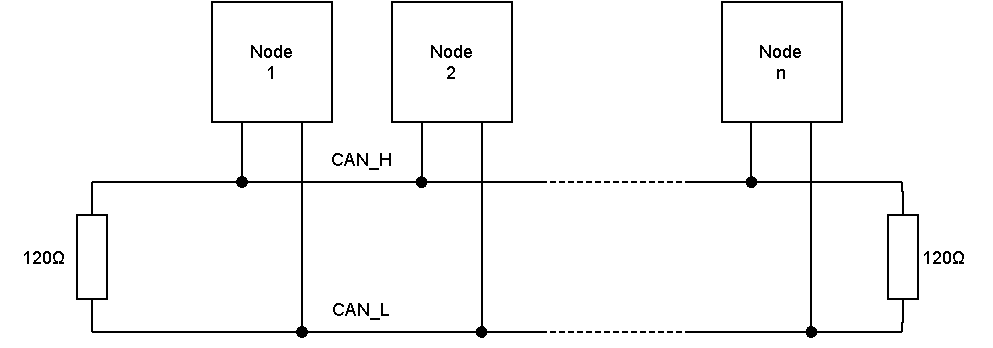
\includegraphics[height=3.8cm]{images/can-bus_topology}
	\caption{Topology of a \acrshort{can}-Bus}
	\label{fig:can-bus_topology}
\end{figure}

As long as the bus is free, any node is allowed to transmit \acrshort{can} messages. Each message is received by all nodes on the network, including the node that sent the message. This type of data broadcasting allows multiple nodes to use the transmitted data. It also allows the sending node to monitor the bus for errors. If two or more nodes try to transmit at the same time, the lower priority message will be overwritten, and this lower priority node will halt transmission upon sensing overwritten bits in its message identifier. The message is then re-transmitted when the bus is again free. This non-destructive process is called bit-wise arbitration.

Every node on the network reads the identifier of a message, and each node independently determines if the message is to be ignored or processed. Since the identifier is specific to the contents of the message rather than the identity of the originating node, new nodes may be added to the network, without modifying the program of any existing node on the network \cite{ti_can_transceivers}.
\newpage

\subsection{Signaling}
The signals on the CAN bus are distinguishes between two bus logic states, dominant and recessive. A recessive bit is defined as CANH being less than CANL + 0.5\,V. A dominant bit is defined as CANH being more than CANL + 0.9\,V. Figure\,\ref{fig:can-signaling} illustrates the nominal case. Since dominant bits overwrite recessive bits, CAN manages message collision through the process of bit-wise arbitration as described earlier.

\begin{figure}[h!]
	\centering
	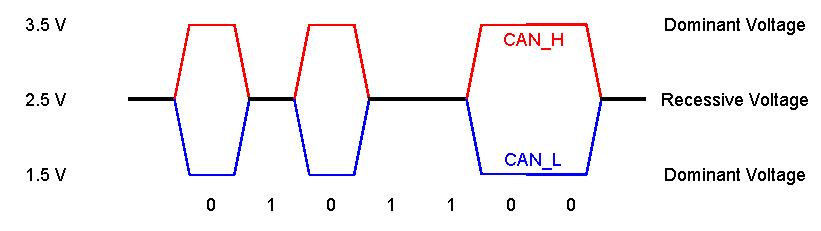
\includegraphics[height=3cm]{images/can-signaling}
	\caption{\acrshort{can}-Bus Signaling}
	\label{fig:can-signaling}
\end{figure}

\subsection{Frames}
Messages over a \acrshort{can} bus are referred to as frames. The most common frame types are defined as \acrshort{can} 2.0A and 2.0B also known as base and extended frame. 2.0A is simply a \acrshort{can} frame with an 11-bit identifier and 2.0B always uses 29-bit. A \acrshort{can} frame is always split up into the following regions \cite{can_bus_tutorial}.

\begin{figure}[h!]
	\centering
	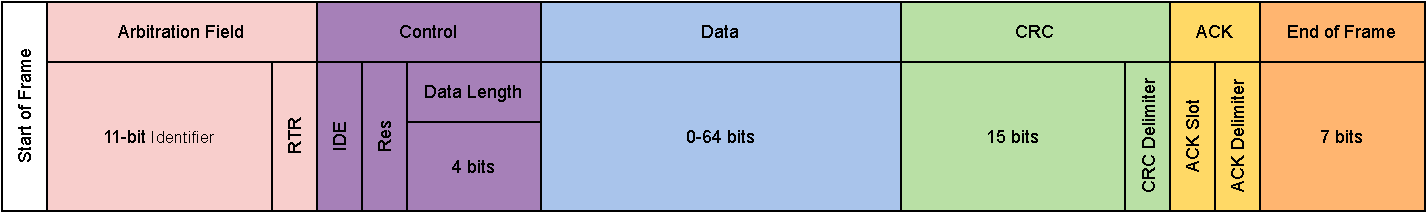
\includegraphics[width=\textwidth]{images/can-frame}
	\caption{Base 11-bit identifier \acrshort{can} frame}
	\label{fig:can-frame}
\end{figure}

\begin{itemize}
		\item The Arbitration Field, includes the identifier of the message and defines the priority. The identifier must be 11 or 29 bits long. Also in this field is the \acrfull{rtr} bit, which is used to request data.
		\item The Control Field is used to differentiate between the two frame types and defines the incoming data length.
		\item The data field can contain 0-8 bytes of information.
		\item The \acrshort{crc} field contains a 15-bit checksum. The checksum is used to detect errors in the transmission.
		\item The Acknowledgement Slot, is used to detect if a message was received by any of the devices on the bus. The transmitter checks for the presence of the Acknowledge bit and re-transmits the message if no acknowledge was detected.
\end{itemize}
\newpage

\section{SAE J1939}
J1939 is the open standard developed by \acrfull{sae}. It is used for networking and communication in the commercial vehicle sector. J1939 is a higher-layer protocol utilizing \acrshort{can} as its physical layer. SAE\,J1939 is primarily a data driven protocol, providing far better data bandwidth than other automation protocols such as \gls{canopen} and \gls{devicenet} \cite{introduction_sae_j1939_protocol}.

The standard specifies CAN bus speeds of 250\,kbit/s or 500\,kbit/s and uses the extended 29-bit identifier frame format. Most messages defined by the J1939 standard are intended to be broadcast only. This means that the data is transmitted on the network without a specific destination. This permits any device to use the data without requiring additional request messages. The 29-bit identifier used in J1939 is structured in the following way \cite{sae_j1939_introduction}. 

\begin{figure}[h!]
	\centering
	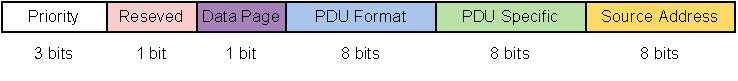
\includegraphics[width=\textwidth]{images/j1939-identifier}
	\caption{29-bit J1939 Identifier}
	\label{fig:29-bit_J1939_Identifier}
\end{figure}
\begin{itemize}
	\item The first three bits of the identifier are used for controlling a message priority during the arbitration process. A value of 0 has the highest priority.
	\item The Reserved bit, Data Page bit, PDU Format field and PDU specific field are often grouped together and referred as \acrfull{pgn}. 
	\item The last 8 bits of the identifier contain the address of the device transmitting the message. Two devices can not share the same address.
\end{itemize}
\newpage

\section{Fleet Management System (FMS)} \label{Fleet Management System (FMS)}
The Fleet Management Systems Interface (FMS) is a standard interface developed by European commercial vehicle manufacturers in 2002. It defines a common interface for telematics applications and include driving as well as diagnostics information. The data is coded according to the SAE\,J1939 standard. FMS is a broadcast only system, a gateway between the internal bus and the FMS bus is implemented by the OEM. 3rd party systems, like the Fleet-Monitor, are forbidden on the internal bus as shown in figure \ref{fig:fms-bus}. 

\begin{figure}[h!]
	\centering
	\hfuzz=14.0pt
	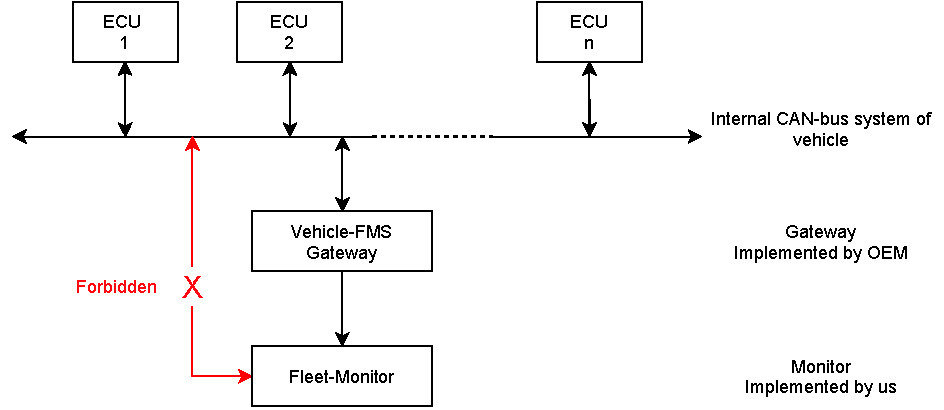
\includegraphics[width=\textwidth]{images/fms-bus}
	\caption{FMS Topology}
	\label{fig:fms-bus}
\end{figure}

At the time of writing, the standard includes 36 different packages, ranging from engine coolant temperature to door position.  Depending on the frame, updates occur between 20\,ms and 10\,s. The convention set the \acrfull{pgn} for J1939 identifiers, while the OEM specify the source address and priority. Each frame has a fixed data length of 8\,byte but not all of them contain information as shown in the example frame bellow.\cite{fms-standard-description}:

\begin{figure}[h!]
	\centering
	\hfuzz=11.0pt
	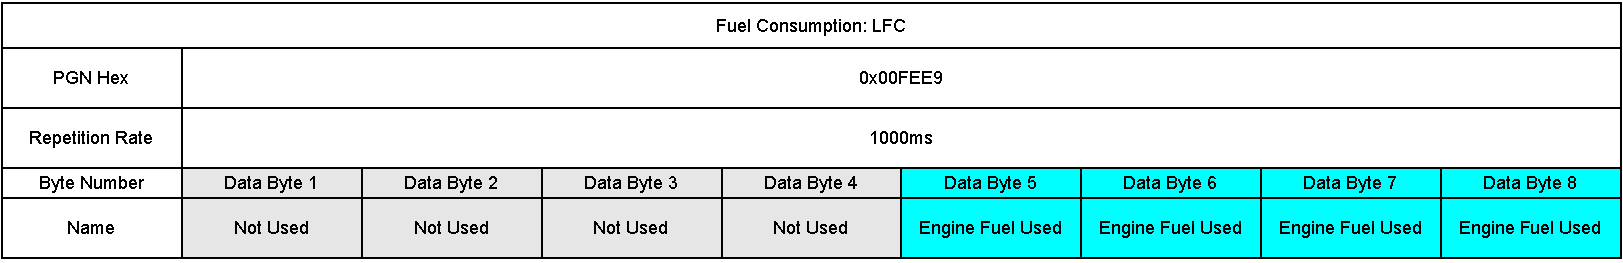
\includegraphics[width=\textwidth]{images/fms-frame}
	\caption{Fuel Consumption FMS Frame}
	\label{fig:fms-frame}
\end{figure}

